\chapter{Algorithms for Computing Tucker2 Decomposition}
\label{chap_algo}

\section{Mathematical Preliminaries}

In this section we recall some mathematical notions
we shall need to discuss the last two algorithms, 
Newton-Grassmann and Differential-Geometric Newton methods.

\subsection{Newton's method}

Let us recall some basic facts about ordinary Newton method. The minimization problem for 
a smooth function is usually reduced to finding zero of the gradient, 
so we shall discuss solving system of equations
$f(x) = 0$, $f \colon \R^n \to \R^n$.

 Geometrically the idea of the method in one-dimensional case is 
to move along the tangent lines to the graph of $f$. Analytically this is expressed by the following iterative formula:
\begin{equation}
 x_{n+1} = x_n - \frac{f(x_n) }{ f'(x_{n})}. 
\end{equation}


\begin{figure}
        \centering
                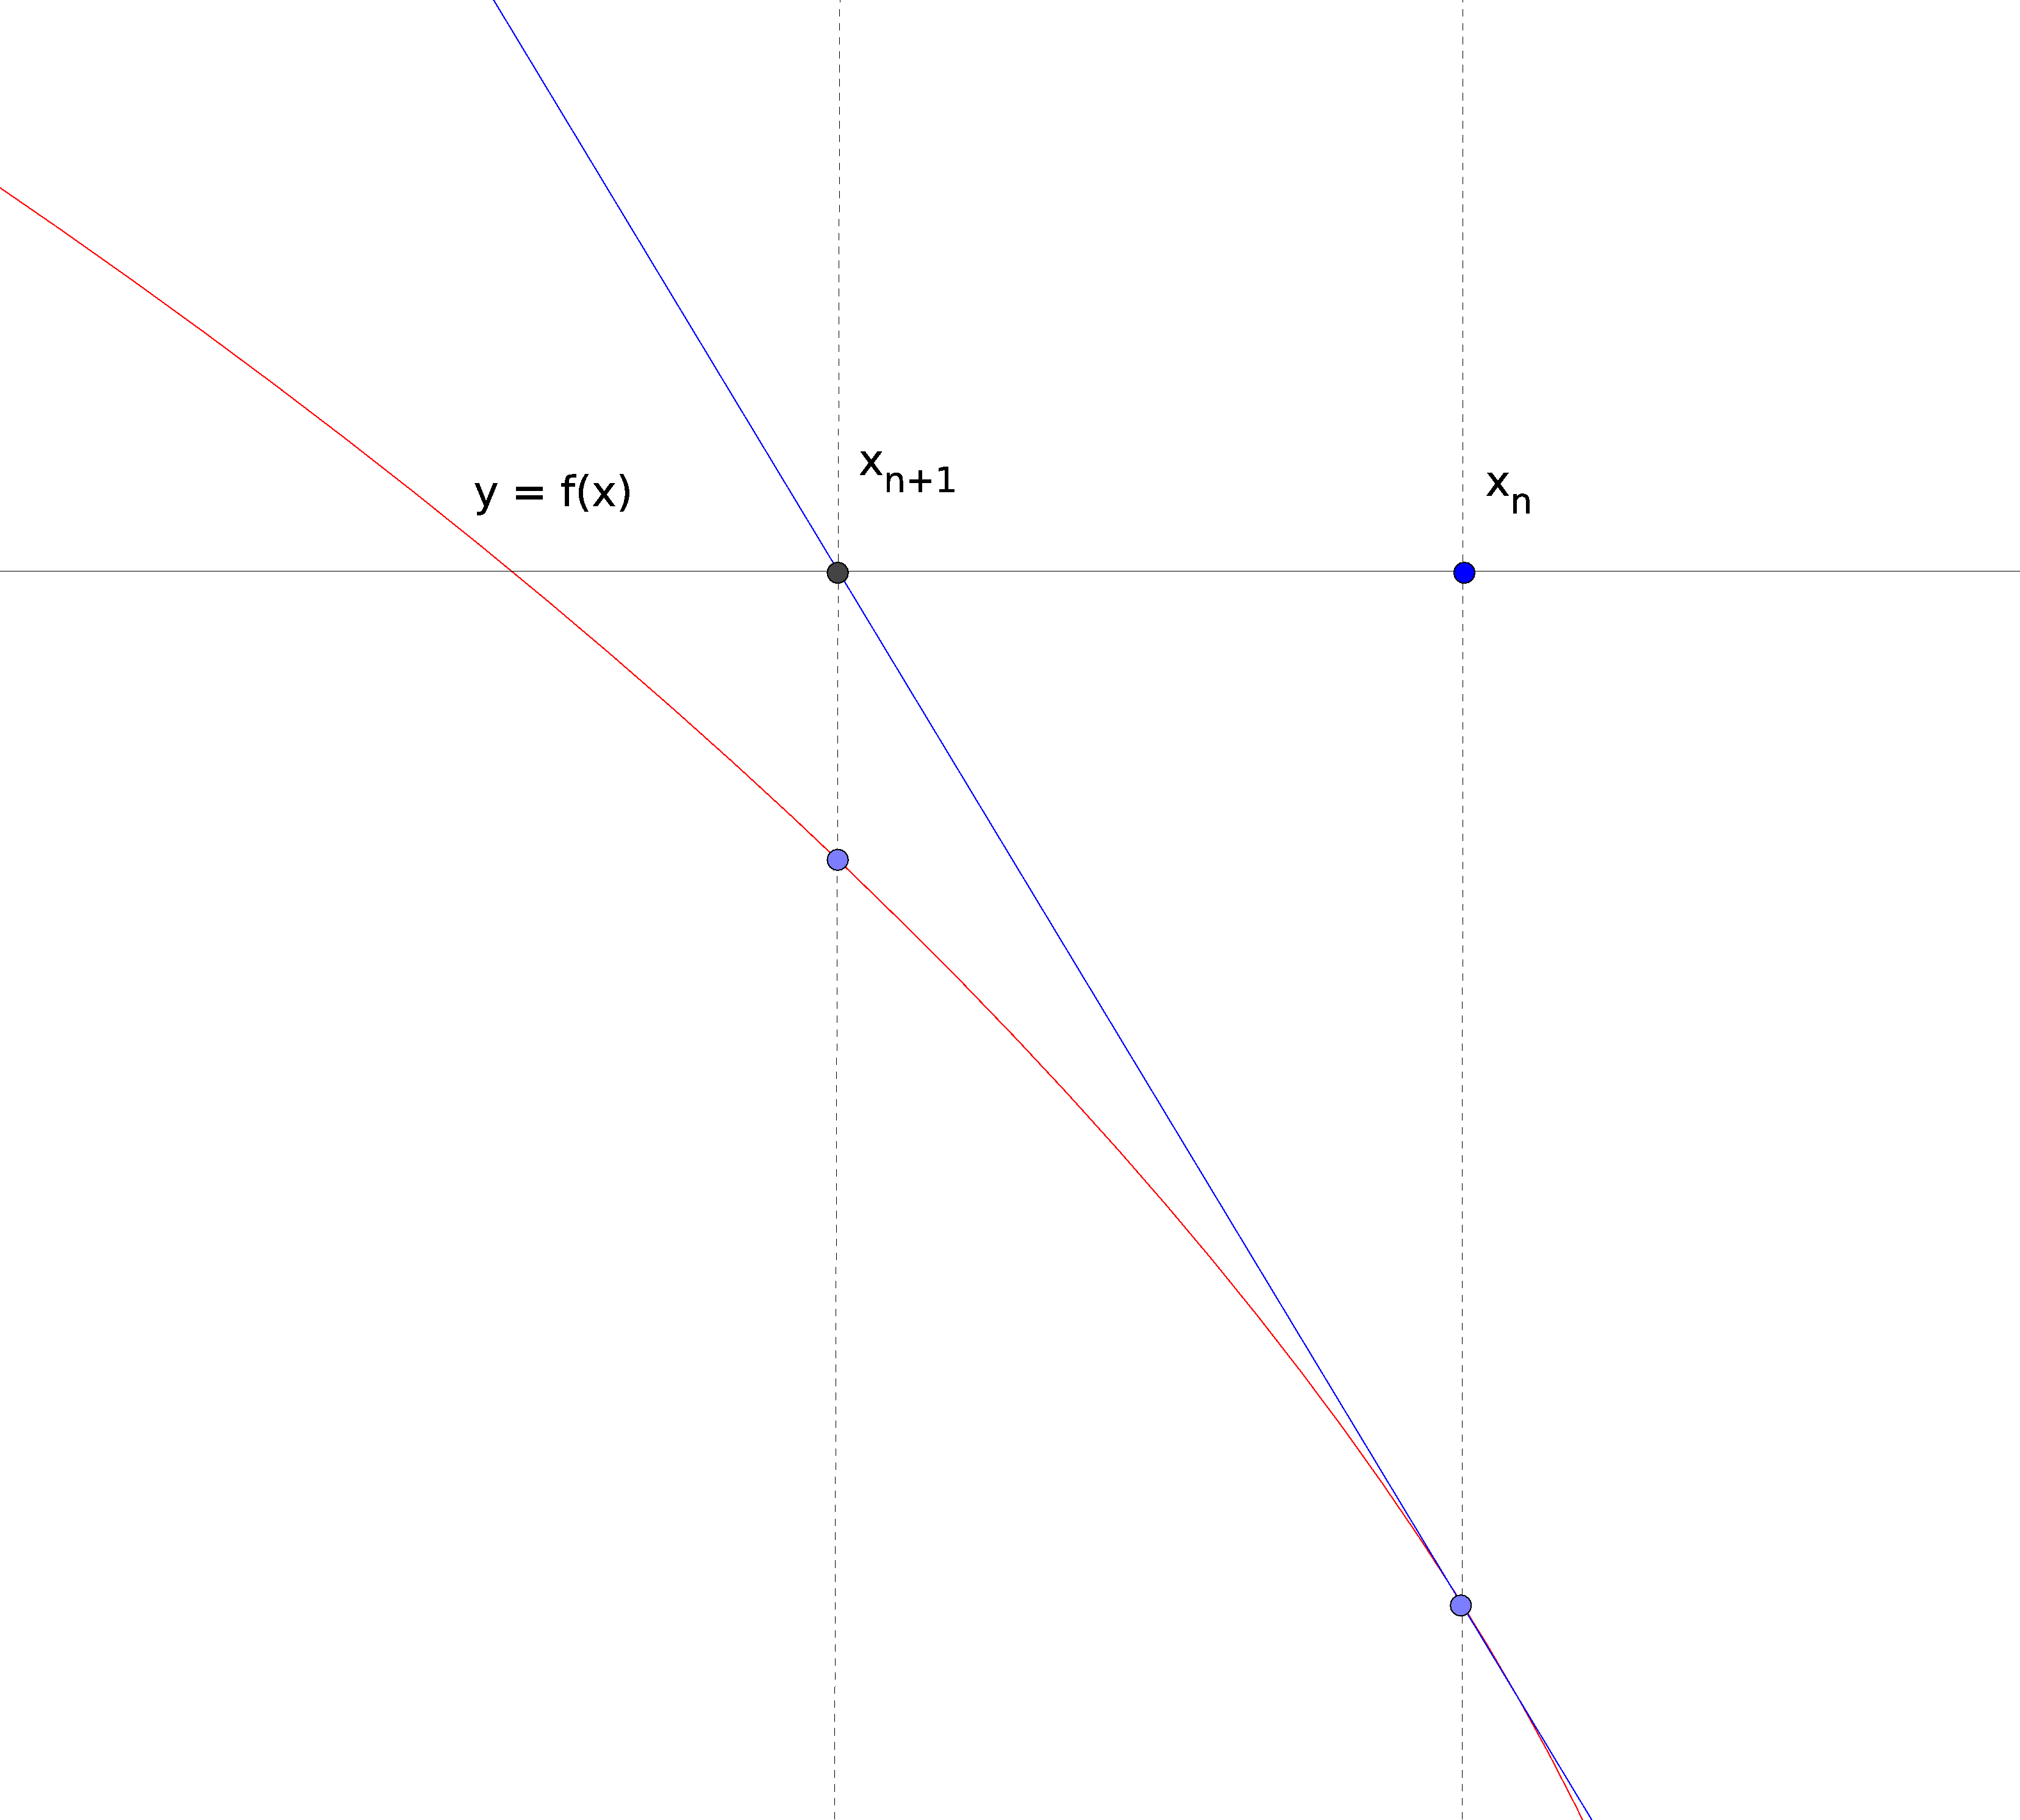
\includegraphics[width=8cm]{images/newton-image1.png}
        \caption{Newton's method illustration}
        \label{fig:hooi_hosvd_comparison}
\end{figure}
The method is known to be very fast-convergent (providing that the initial value $x_0$ is close enough to a root).
In multidimensional case the formula is
\begin{equation}
 x_{n+1} = x_n - ((Df)(x_n))^{-1} ( f(x_n) ).
\end{equation}
Here $(Df)(x_n)$ denotes the Jacobi matrix of the mapping $f$. In practice, instead of finding
the inverse of this matrix and then applying it to the vector $f(x_n)$, it is 
easier to solve the linear system $(Df)(x_n) y = f(x_n) $, but still this step is computationally expensive,
especially if the number of variables is high.


If we use this method to minimize $F$ by finding the zero of $\nabla F$, then
we can also interpret this method in terms of $F$. If we approximate $F$
with its Taylor expansion of degree $2$, then in a neighbourhood 
of a non-degenerate extremum point the level sets will be ellipses.
The gradient is known to be orthogonal to level set, so, if we use gradient descent,
we may come to the optimum quite slowly, if the ellipses are very elongated.
The Newton's method involves inverting of $D (\nabla F)$, that is, inverting 
the Hessian of $F$, which is exactly the quadratic part of the Taylor expansion.
By inverting it we essentially transform our problem to a coordinate system in which
the level sets are circular and this allows us to move to the optimum much faster (see Figure \ref{fig:newt_grad_comp}).

\begin{figure}
        \centering
                
\includegraphics[width=4cm]{images/newton_vs_grad_desc.jpg}
        \caption{Newton's method illustration}
        \label{fig:newt_grad_comp}
\end{figure}


However, Newton's method is known to behave poorly, if the root is not isolated.
This is exactly the situation we have in Tucker2 decomposition, where the objective function
does not change, if factor matrices are multiplied by any orthogonal matrices. The geometric
interpretation of this operation is that we choose another orthonormal basis in the same subspace.
There are orthogonal matrices approximately close to the identity matrix, so the zeros
of gradient w.r.t. entries of $F_2$, $F_3$ are not isolated. In order to apply Newton's method
we need to work in more geometric terms, and we start by brief informal description of the notions
that are necessary, namely: smooth manifold, tangent space, differential of a mapping between two smooth manifolds,
Riemannian metric, geodesic.
We are not going to give 
rigorous mathematical definitions, otherwise it would be necessary
to reproduce a significant part of several mathematical textbooks.
Instead we give a very informal description, which should be sufficient
to understand the intuition behind the two remaining methods.


\subsection{Some notions from differential geometry}
A smooth manifold of dimension $n$ is a space which locally 
looks like $\R^n$. 
This means that in a neighbourhood of each point we have a local coordinate system $(x_1(\cdot), \dots,  x_n(\cdot))$.
Point $p$ of a manifold $M$ in this system is described by $(x_1(p), \dots, x_n(p)) \in \R^n$. Usually these coordinate systems 
cover only a part of the manifold, but each point belongs to the domain
of at least one of them.
If the domains of two coordinate systems $(x_1(\cdot), \dots, x_n(\cdot))$
and $(y_1(\cdot), \dots, y_n(\cdot))$ intersect, then we have transition functions
\begin{equation}
(x_1, \dots, x_m) \mapsto (y_1, \dots, y_n) \mbox{ if } \exists p : x_i(p) = x_i \mbox{ and } y_i(p) = y_i \mbox{ for all } i.
\end{equation}
These functions must be differentiable (this is a part of the definition of smooth manifold).
This approach to manifolds does not require them to be a subset of 
any ambient Euclidean space $\mathbb{R}^N$. There is Whitney's embedding theorem 
that states that any manifold can be embedded into $\mathbb{R}^N$
for some $N$. However, sometimes there is no good or natural way to choose this embedding.
Examples.
\begin{enumerate}
    \item $\R^n$ is a manifold (the identity mapping is a coordinate system that
        covers the whole space). Since every finite-dimensional vector space is 
        isomorphic to $\R^n$, vector spaces are also manifolds. In particular,
        the space of $m \times n$ matrices is a manifold isomorphic to $\R^n$.
    \item If $M$ is a manifold, then every open subset of $M$ is also a manifold.
        In particular, the set of $m \times n$ matrices with some fixed rank $k$
        is a manifold. We shall need the set $\R^{n \times n}_{*}$ of non-singular $n \times n$ matrices,
        which is a manifold by this remark.
    \item If $M$ is a smooth manifold and there is an equivalence relation $\sim$ on $M$,
        then, under some conditions, the set of equivalence classes $M / \sim$ is 
        also a manifold (\textit{quotient manifold theorem}, see \cite{lee_manifolds}).
    \item If $M$ and $N$ are smooth manifolds, then $M \times N$ is a smooth
        manifold.
\end{enumerate}


Let $p$ be an arbitrary point of a smooth manifold $M$. The tangent space at $p$
is a vector space of the same dimension as $M$ and it is denoted by $T_pM$.
Suppose that for each point $p \in M$ we choose one vector $X_p \in T_pM$. 
This gives us a mapping $X: M \to \cup_{p \in M} T_pM$ called a
\textit{vector field on $M$}.


The notion of a tangent space is intuitively clear if we think about something like a sphere.
However, if $M$ is an open subset of $\R^n$, the tangent space at each point
is also $\R^n$.
\begin{equation}
    \forall p \in \R^n \quad T_p\R^n = \R^n.
\end{equation}
We shall often use this in the discussion of Newton methods, because
it allows us to treat matrix-valued functions of matrix argument $\R^{m \times n} \to \R^{m \times n}$
as vector fields on the manifold of matrices ($\R^{m \times n} \cong \R^{mn}$ as vector spaces).


Generally speaking, the only structure that $T_pM$ has is that of a vector space, there is no
inner product and there is no correspondence between $T_pM$ and $T_qM$ for different
points $p, q \in M$. However, this structure is sufficient to define a differential
of a mapping between two smooth manifolds. Let $f : M \to N$ be a smooth
function between smooth manifolds $M$ and $N$ (this means that, if we write
$f$ in local coordinates on some part of $M$ and the corresponding part of $N$,
we get a smooth function of real arguments). The differential of $f$
at point $p \in M$ is a linear operator $(Df)_p : T_pM \to T_{f(p)}N$ which in
local coordinates is given by the Jacobi matrix. In particular,
if $f : M \to \R$ is a smooth real-valued function on $M$, its differential at point $p$,
called \textit{gradient} is a linear functional on $T_pM$,
so the gradient of a function is not a vector (element of a tangent space),
but a covector (element of an adjoint space $(T_pM)^*$).



If each $T_pM$ is equipped with an inner product
that changes smoothly as we move along $M$, then $M$ is said to be a Riemannian manifold.
A smooth curve on $M$ is a smooth mapping $\gamma : [a, b] \rightarrow M$.
Its differential at point $p \in (a, b)$ is a linear mapping $(D\gamma)(p) : T_p(a,b) \to T_pM$.
By the previous remark, $T_p(a, b) = T_p \R = \R$, and we can calculate $(D\gamma)_p(1) \in T_pM$.
This element of $T_pM$ is called \textit{velocity vector}, and we can calculate
its Euclidean norm using the inner product in $T_pM$. This defines a real-valued function
on $(a, b)$. By definition, the length of the curve $\gamma$ is the integral
of this function over $(a,b)$, so the Riemannian structure allows us to measure curves on $M$.


Moreover, if $T_pM$ has an inner product, then there is a natural isomorphism
between $T_pM$ and its adjoint space $(T_pM)^*$. This means that the 
gradient of a function on a Riemannian manifold can be viewed as a vector (element
of $T_pM$).


If two different points $p, q$ on a Riemannian manifold are close enough to each other,
there is a unique shortest path connecting $p$ and $q$. 
The condition of being locally shortest path is certain differential equation
and it's solutions are called geodesics. If we consider $S^2$ in $\mathbb{R}^3$, 
then geodesics are arcs of large circles. This example illustrates that in general it is not true,
that two points are connected by the unique geodesics (consider North and South poles)
or that geodesic path is always the shortest: if $p$ and $q$ are close to each other,
there is a unique large circle passing through $p$ and $q$, but it gives rise to two
geodesics: the shortest path is the shorter arc of the circle, but the longer arc 
is a geodesic, too.


In the differential-geometric Newton method
we shall need the notion of fiber bundle.
We start with two toy examples.
A cylinder $ \{ (x, y, z) \mid x^2 + y^2 = 1, 0 \leq z \leq 1 \}$
can be split into disjoint copies of $[0,1]$ (generating lines)
parameterized by the base $\mathbb{S}^1$,
so there is one instance of $[0,1]$ attached to each point of the circle.
A M\"obius band can also be split into disjoint segments
$[0,1]$ parameterized by $\mathbb{S}^1$. Locally both the cylinder
and M\"obius band are isomorphic to a cartesian product
of the arc of a circle and $[0,1]$. The cylinder is, of course,
isomorphic to the cartesian product not just locally, but globally,
but it is not the case for the M\"obius band, where the trivial
 pieces are glued together in a non-trivial way. Both these spaces
are called total spaces of fiber bundles with the base $\mathbb{S}^1$ and fiber $[0,1]$.
Another example of a fiber bundle is a torus $\mathbb{S}^1 \times \mathbb{S}^1$,
where both the base and the fiber are circles. 

In general, a fiber bundle is a triple $( \pi, E, B)$, where
$ \pi \colon E \to B$ is a surjective mapping such that:
\begin{enumerate}
    \item The inverse image $\pi^{-1}(p)$ of each point $p \in B$ is 
    isomorphic to some fixed manifold $F$.
    \item Every point $p \in B$ has a neighbourhood $V_p$
    such that $\pi^{-1}(V_p)$ is isomorphic to $V_p \times F$.
\end{enumerate}
    The space $E$ is a \textit{total space} of the bundle, $B$ is a textit{base}, and $F$ is a \textit{fiber}.

Since the tangent space is a local notion, for each point $p \in E$
the tangent space at $p$ is isomorphic to a direct product
of the tangent space to the base $T_h$ and the tangent space to the fiber $T_v$,
\begin{equation}
    T_p E = T_h \oplus T_v
\end{equation}
If one wants to visualize a fiber bundle,
one usually thinks of the base positioned horizontally and the fibers
attached to the base in the orthogonal (that is, vertical) direction,
therefore the space $T_h$ is called a horizontal space and the space $T_v$
is called a vertical space.

\begin{figure}
        \centering
                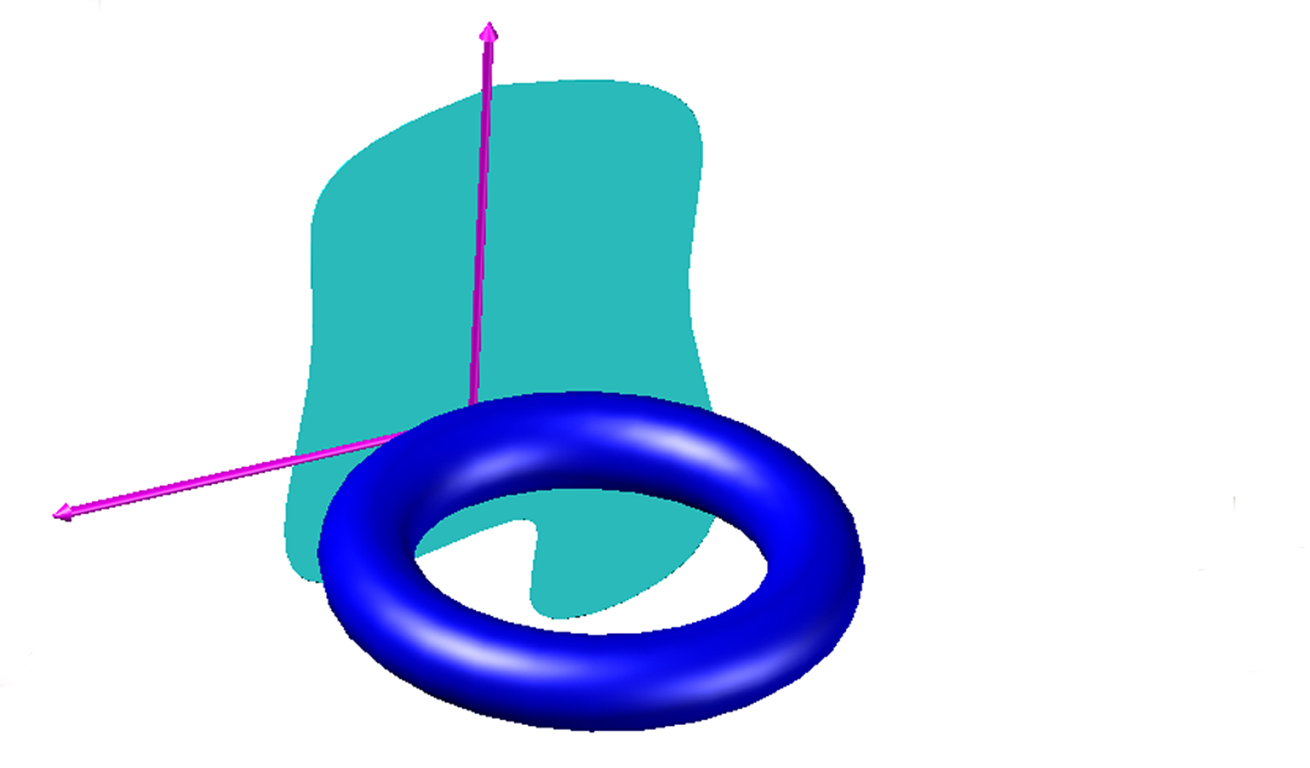
\includegraphics[width=8cm]{images/torus_tangent.jpg}
        \caption{Tangent plane to a fiber bundle}
        \label{fig:torus_tangent}
\end{figure}


The last notion we shall describe here is \textit{affine connection on a manifold}.

We say that $\nabla$ is an affine connection on a manifold $M$,
if for each vector field $X$ on $M$ we have an operator $\nabla_X$ that
maps vector fields to vector fields on $M$ and satisfies 
the following axioms:
\begin{enumerate}
    \item $\nabla_X$ is an $\R$-linear operator;
    \item (Leibniz formula) $$\nabla_X(fY) = (Xf) \cdot Y + f \nabla_X Y $$
        Recall that, if $X = \sum_k b_k \frac{\partial}{\partial x_k}$ is a coordinate representation 
        of vector field $X$, then the function
        $Xf$ is defined by
        $$Xf = \sum_k b_k \frac{\partial f}{\partial x_k}$$
    \item $$ \nabla_{X + Y} = \nabla_X + \nabla_Y $$
        and
        $$ \nabla_{fX} = f \nabla_X.$$
\end{enumerate}
The field $\nabla_{X} Y$ is called the covariant derivative of $Y$ along $X$.
This operation is a generalization of differentiation in $\R^n$.
It plays a central role in differential geometry,
capturing the properties of curved spaces. In particular,
with affine connection it is possible to perform
parallel translation of a vector along a curve, so
affine connections 'connect' tangent
spaces at different points.




\section{Higher-order SVD}
\label{sec_hosvd}

This method is analogous to standard method of computing PCA for matrices.
Recall that if $A$ is an $m \times n$ real matrix, then it can be decomposed as 
\begin{equation}
\label{svd_def}
 A = U \Sigma V^T,
\end{equation}
where $\Sigma$ is a (rectangular) diagonal matrix with non-negative elements on the diagonal and $U$ and $V$ are orthogonal matrices: $U \in O(m)$, 
$V \in O(n)$. $U$ is called the matrix of left singular vectors (its columns are eigenvectors of $AA^T$), $V$ is the
matrix of right singular vectors (eigenvectors of $A^TA$). Let $ \sigma_1 \geq \dots \geq \sigma_r$ be non-zero diagonal elements of $\Sigma$, then the rank of $A$ is $r$. The decomposition \eqref{svd_def} 
is called Singular Value Decomposition (SVD). The optimization problem
\begin{equation}
\| A - B \| \to \min \mbox{ subject to $\rk B = k $}
\end{equation}
is a matrix analog of Tucker \eqref{tucker_min}. Unlike tensor case, this problem can be solved exactly.
Let $\Sigma_k$ be  the matrix obtained from $\Sigma$ by setting $\sigma_{k+1}, \dots, \sigma_r$
to $0$, then the optimal matrix $B$ is $U \Sigma_k V^T$. 

The higher-order singular value decomposition for Tucker2 is formulated as follows.


\begin{algorithm}
\caption{HOSVD}\label{HOSVD}
\begin{algorithmic}[1]
\Function{HOSVD}{ $\A \in \R^{d_1 \times d_2 \times d_3}$, $r_2$, $r_3$}

\State Compute SVD of unfoldings $\A_{(2)}$ and $\A_{(3)}$:

\begin{eqnarray}
 \A_{(2)} = U_2 \Sigma_2 V_2^T  \\
 \A_{(3)} = U_3 \Sigma_3 V_3^T
\end{eqnarray}

\State Truncate matrices of left singular vectors $U_2$ and $U_3$ and take the result
as projection matrices $F_2$, $F_3$.

\begin{eqnarray}
F_2 = U_2(:, 1:r_2) \\
F_3= U_3(:, 1:r_3)
\end{eqnarray}


\State \Return $F_2$, $F_3$

\EndFunction
\end{algorithmic}
\end{algorithm}



This method is a heuristic, there is no mathematical proof that it gives
the approximation which is in some sense 'good'. However, in practice this produces
results that are reasonable and is used as initialization for iterative methods.

\section{Higher-order Orthogonal Iteration (HOOI)}

Next algorithm is Higher-Order Orthogonal Iteration (HOOI). (see~\cite{kolda_bader_2009}).
This algorithm is a special case of alternating least squares.
In one iteration of this method we fix $F_2$ and optimize the cost function for the other factor matrix $F_3$,
then fix $F_3$ and solve the optimization problem for $F_2$. 
The advantage of this procedure is that optimization for one factor matrix can be solved exactly
by SVD, as mentioned earlier. The pseudocode form of the algorithm is

\begin{algorithm}
\caption{HOOI}\label{HOOI}
\begin{algorithmic}[1]
\State Initialize $F_2$, $F_3$ using HOSVD
\Repeat 


$\mathcal{B} := \A \times{_3} F_3^T$
    
    
$\mathcal{C} := \A \times{_2} F_2^T$
    
    
$F_2 := d_2 \mbox{ leading left singular vectors of }{\mathcal{B}}_{(2)}$
    
    
    $F_3 := d_3 \mbox{ leading left singular vectors of }{\mathcal{C}}_{(3)}$
\Until termination criterion satisfied or maximum iterations exhausted.
\end{algorithmic}
\end{algorithm}


There are several standard options for termination criterion.
We may require that the norm of the residual is below
some predefined threshold,
\begin{equation}
    R := \| \A - \A \times_2 F_2^T \times_3 F_3^T \| \leq \epsilon,
\end{equation} 
or we may consider the relative norm,

\begin{equation}
    \frac{R}{\| \A \| } \leq \epsilon.
\end{equation} 


Another option would be to stop when the norm or the relative norm of the gradient of the objective
function $\Phi$ gets small enough,
\begin{eqnarray}
    \| \nabla \Phi \| \leq \epsilon \mbox{ or}\\
    \frac{ \| \nabla \Phi \|  }{\| \A \| } \leq \epsilon.
\end{eqnarray} 
The compact formula for the gradient will be given in the section on Newton-Grassmann
method (formula \eqref{grad_phi}). It is important to use the projected
gradient here, the formal gradient (vector of partial
derivatives with respect to the elements of $V$ and $W$, its compact
representation is given in the formula \eqref{formal_grad_phi})
increases as we run the iterations, due to the 
orthogonality constraints.
It is also possible to stop iterations when there is no further improvement. 
For example, let $R_k$ be the norm of the residual
at the {$k$th} iteration. We keep iterating as long as  $R_k \leq R_{k-1} - \epsilon$.


\section{Newton-Grassmann method}

This method was introduced by Elden and Savas. 
The general scheme of the method is as follows.
Let $\Phi \colon M \to \R$ be a smooth function 
on a Riemannian manifold $M$, we want to maximize $\Phi$.
Let $p \in M$
be a current approximation. The function $\Phi$ has the gradient 
$\nabla \Phi (p) \in T_pM$ and the Hessian $H(\Phi)_p$
which can be interpreted as a linear operator on $T_pM$.
If $p$ is close enough to the point of maximum of $\Phi$,
the Hessian is non-singular, and there exists a unique tangent vector 
$\Delta \in T_pM$ that satisfies the equation
\begin{equation}
    \label{NewgrGeneral}
    H(\Phi)_p(\Delta) = - \nabla \Phi(p).
\end{equation}
This vector defines the geodesic curve $t \mapsto \gamma(t)$ on $M$,
and we move along it to find the next approximation to the solution,
\begin{equation}
p_{+} = \gamma(1).
\end{equation}


The manifold on which the method by Elden and Savas works is the product
of \textit{Grassmann manifolds}, and we start with its definition and basic properties.  Let $k \leq n$ be positive integers. We interpret the manifold $St(n, k)$
of $n \times k$ matrices with orthonormal columns
as the set of orthonormal basises of $k$-dimensional subspaces
of $\R^n$. Two matrices $X$ and $Y$ represent the same subspace,
if there exists an orthogonal $k \times k$ matrix $U$ such that
$X = YU$. This defines an equivalence relation $\sim$ on $St(n, k)$. The quotient $St(n, k)/ \sim$ is called
Grassmann manifold and denoted $Gr(n, k)$.
Let $[X] \in Gr(n,k)$ be an equivalence class of matrix $X$.
It is known that the tangent
space $T_{[X]}Gr(n, k)$ can be identified with the set of matrices $\Delta$
such that 
\begin{equation}
    X^T \Delta = 0
\end{equation}
Let $\Pi$ be an operator
\begin{equation}
    \Pi_X(W) = W - XX^TW
\end{equation}
This operator projects $\R^{n \times k}$ onto $T_XGr(n, ,k)$. Indeed,

\begin{equation}
    X^T \Pi_X(W) = X^T W - X^TXX^T W = X^TW - X^TW = 0,
\end{equation}
since $X$ has orthonormal columns, that is, $X^TX = I$.


The canonical inner product in $T_X Gr(n, k)$ is defined by
\begin{equation}
    \langle \Delta_1, \Delta_2 \rangle := \tr( \Delta_1^T \Delta_2).
\end{equation}
Equipped with this inner product, $Gr(n, k)$ becomes a Riemannian
manifold. The formula
for the geodesic curve that passes through $X$ at $t = 0$ and has at this point tangent 
vector $\Delta$ is 
\begin{equation}
    X_{\Delta}(t) = XV \cos (t \Sigma) V^T + U \sin(t \Sigma) V^T,
\end{equation}
where $U \Sigma V^T$ is the thin SVD of $\Delta$.


In the sequel we shall abuse the notation by identifying $[X] \in Gr(n, k)$
and its representative $X \in \R^{n \times k}$. Functions $F$
on $Gr(n, k)$ will be interpreted as functions on $St(n, k)$ with the additional
symmetry property
\begin{equation}
    \label{sym_grass}
    \forall U \in O(k) \quad F(XU) = F(X).
\end{equation}
Since $St(n,k)$ can be identified with the subset of $\R^{nk}$, we can compute
the \textit{formal gradient} of $F$ by taking partial derivatives of $F$
with respect to all entries of the argument $X$. Let this gradient
be $F_X(X)$, then the gradient of $F$ as a function on Grassmannian
is computed by projecting:
\begin{equation}
\nabla F (X) = \Pi_{X} F_X(X).
\end{equation}

We noticed before that the objective function in Tucker2 decomposition 
problem
\begin{equation}
\Phi(F_2,F_3) = \frac{1}{2} \| \A \times _{2} F_2 \times _{3} F_3 \| 
\end{equation}
satisfies the symmetry property \eqref{sym_grass} w.r.t. both arguments,
so we can interpret it as a function on $M = Gr(d_2, r_2) \times Gr(d_3, r_3)$.
We start with computing its gradient. 

%Recall that for any function $f$ the linear part of $ f(x(t)) - f(x(0)) $ is equal to $ \langle \Delta, \nabla f \rangle $,
%where $\Delta$ is the tangent vector to the curve $x(\cdot)$ at $0$. We shall use this property 
%to calculate the gradient of $\Phi$.

Let ${F_2}(t)$ and ${F_3}(t)$ be arbitrary curves on $Gr(d_2, r_2)$
and $Gr(d_3, r_3)$, $\Delta_2$ and $\Delta_3$ be the corresponding tangent
vectors at $t = 0$.
If we derive the representation of $\frac{d \Phi(F_2(t), F_3(t))}{dt} \rvert_{t = 0}$ in the form
$\langle \Delta, \Theta \rangle$, where $\Delta$ is a tangent vector
to the curve $t \mapsto (F_2(t), F_3(t))$ on $St(d_2, r_2) \times St(d_3, r_3)$ 
at $t = 0$, then the vector $\Theta$ will be the formal gradient of $\Phi$.
Since the tangent space to the product of two Riemannian manifolds is
isomorphic to the product of tangent spaces (as inner product spaces), we
have $\Delta = (\Delta_2, \Delta_3)$, $\Theta = (\Theta_2, \Theta_3)$
and $\langle \Delta, \Theta \rangle = \langle \Delta_2, \Theta_2 \rangle + 
\langle \Delta_3, \Theta_3 \rangle $.


%\begin{equation}
%\frac{d}{dt}\left(A \times _k X(t) \times _m {F_2}(t) \right) = A \times_k \frac{d}{dt}(X(t)) \times _m {F_2}(t) + A \times_k  X(t) \times _m \frac{d}{dt}({F_2}(t))
%\end{equation}
%Here $A$ is a constant tensor and $X(t)$ and ${F_2}(t)$ are matrix-valued functions of $A$.

Using the Leibniz formula, we obtain
\begin{equation}
\begin{split}
\frac{d\Phi(F_2(t), F_3(t))} {dt} &= \frac{1}{2} \frac{d}{dt} \langle \A \times_2 F_2(t) \times_3 F_3(t), \A \times_2 F_2(t) \times_3 F_3(t) \rangle   \\
 &= \langle \A \times_2 \Delta_2 \times_3 F_3, \A \times_2 F_2 \times_3 F_3 \rangle  \\ 
 & +  \langle \A \times_2 F_2 \times_3 \Delta_3 , \A \times_2 F_2 \times_3 F_3 \rangle 
 \end{split}
\end{equation}

Let
\begin{equation}
\G := \A \times_2 {F_2} \times_3 {F_3}.
\end{equation}

Using formulae from \cite{elden_savas_2007}, we get

\begin{eqnarray}
\langle \A \times_2 \Delta{_2} \times_3 {F_3}, F \rangle = \langle \Delta{_2}, \langle  \A \times_3 {F_3}, F \rangle _{-2} \rangle, \\
\langle \A \times_2 {F_2} \times_3 \Delta{_3}, F \rangle = \langle \Delta{_3}, \langle  \A \times_2 {F_2}, F \rangle _{-3} \rangle.
\end{eqnarray}

This shows that the formal gradient of $\Phi$ consists of two components $(\Phi_2, \Phi_3)$
given by

\begin{eqnarray}
\label{formal_grad_phi}
\Phi{_2} := \langle  \A \times_3 {F_3}, F \rangle _{-2} \\
\Phi{_3} := \langle  \A \times_2 {F_2}, F \rangle _{-3}
\end{eqnarray}

Now we need to project to get $\Phi$, the $\Phi_2$ component is projected to $T_{F_2}Gr(d_2, r_2)$ and
the $\Phi_3$ component is projected to $T_{F_3}Gr(d_3, r_3)$. Omitting the intermediate calculations,
we give the final result ($\Pi_i$ stands for $\Pi_{F_i}$ ):

\begin{equation}
\label{grad_tucker2}
\nabla \Phi = 
\begin{pmatrix}
\Pi{_2} \Phi{_2} \\
\Pi{_3} \Phi{_3}
\end{pmatrix} 
=
\begin{pmatrix}
\langle \A \times_3 {F_3}, \A \times_3 {F_3} \rangle_{-2}{F_2} - {F_2} \langle F, F \rangle_{-2} \\
\langle \A \times_2 {F_2}, \A \times_2 {F_2} \rangle_{-3} {F_3} - {F_3} \langle F, F \rangle_{-3}
\end{pmatrix}
\end{equation}

Next step is to compute the Hessian $H$. Since $\Phi$ is defined on the product
of two manifolds, the Hessian $H$ has the block structure
\begin{equation}
    H = \begin{pmatrix}
        H_{2,2} & H_{2,3} \\
        H_{3,2} & H_{3,3} \\
    \end{pmatrix}
\end{equation}
Here $H_{i,j}$ is a linear operator from $T_{F_j}Gr(d_j, r_j)$ to $T_{F_i}Gr(d_i, r_i)$.
Since $H$ is a self-adjoint operator, $H_{2,3} = H_{3,2}'$.


We again start from computing Hessian
w.r.t. elements of $F_2$ and $F_3$, then we shall need to apply projection 
operator to get $H$. From standard calculus in $\R^n$ we know that
Hessian can be characterized as the linear operator $H$ such that
\begin{equation}
\frac{d^2 \Phi(F_2(t), F_3(t))}{dt} \rvert_{t = 0} = \langle \Delta, H \Delta \rangle.
\end{equation}
Calculate the second derivative of $\Phi(F_2(t), F_3(t))$:
\begin{eqnarray*}
\frac{d^2 \Phi}{dt^2} = \langle \A \times_2 \Delta{_2} \times_3 {F_3}, \A \times_2 \Delta{_2} \times_3 {F_3} \rangle 
+ \langle \A \times_2 \Delta{_2} \times_3 {F_3}, \A \times_2 {F_2} \times_3 \Delta{_3} \rangle \\
+ \langle \A \times_2 \Delta{_2} \times_3 \Delta{_3}, F \rangle 
+ \langle \A \times_2 {F_2} \times_3 \Delta{_3}, \A \times_2 \Delta{_2} \times_3 {F_3} \rangle \\ 
+ \langle \A \times_2 {F_2} \times_3 \Delta{_3}, \A \times_2 {F_2}  \times_3 \Delta_{F_3} \rangle 
+ \langle \A \times_2 \Delta{_2} \times_3 \Delta{_3}, F \rangle 
\end{eqnarray*}

Consider the $(2,2)$-term:

\begin{eqnarray*}
\langle \A \times_2 \Delta{_2} \times_3 {F_3}, \A \times_2 \Delta{_2} \times_3 {F_3} \rangle \\
= \langle \Delta{_2}, \langle \A \times_3 {F_3}, \A \times_2 \Delta{_2} \times_3 {F_3} \rangle_{-2} \rangle \\
 = \langle \Delta{_2}, \langle \A \times_3 {F_3}, \A  \times_3 {F_3} \rangle_{-2} \Delta{_2} \rangle
\end{eqnarray*}

This gives the $(2,2)$-term of the Hessian in operator form:

\begin{equation}
H_{2,2}(\Delta{_2}) = \Pi{_2} \langle \A \times_3 {F_3}, \A \times_3 {F_3} \rangle_{-2} \Delta{_2} - \Delta{_2} {F_2}^T \Phi{_2}
\end{equation}

In the same way the $(3,3)$-term is

\begin{equation}
{H}_{3,3}(\Delta{_3}) = \Pi{_3} \langle \A \times_2 {F_2}, \A \times_2 {F_2} \rangle_{-3} \Delta{_3} - \Delta{_3} {F_3}^T \Phi{_2}
\end{equation}

The $(2,3)$-term is a bit more tricky to compute.

\begin{equation}
H_{2,3}(\Delta{_3}) = \Pi{_2} \left( \langle  \langle \A, F \rangle_{-(2,3)}, \Delta{_3} \rangle_{2,4;1,2}    
+ \langle \langle \A \times_3 {F_3}, \A \times_2 {F_2} \rangle_{-(2,3)}, \Delta{_3} \rangle_{4,2;1:2} \right)
\end{equation}

Until now it was sufficient to work with $T_F Gr(d,r)$ as a subspace of  $\R^{d \times r}$.
However, the elements of $\Delta_2$, $\Delta_3$ are not linearly independent:
the condition $F_i^T \Delta_i = 0$ imposes additional linear constraints,
so it would be unwise to use the elements of these matrices as unknowns
in the final system of equations. We want a non-singular system
with the same number of equations and unknowns. There is a more explicit description
of $T_F Gr(d, r)$ that allows us to do this.  For a $d \times r$ ($d > r$) matrix
$F$ with orthonormal columns we can always find a (non-unique) matrix $F^{\bot}$ such that $[ F \, F_{\bot} ]$
is an orthogonal $d \times d$ matrix (in more geometric terms, we extend the orthonormal
basis of the subspace to the ortonormal basis of the whole space). It turns out that
$\Delta = F^{\bot} D$, $D \in \R^{(d-r) \times r}$ is the appropriate parametrization
of $T_F Gr(d, r)$.

Let us fix some
$F_{2}^{\bot}$ and $F_3^{\bot}$. Then, for $D_i \in \R^{(d_i - r_i) \times r_i}$
we have
\begin{eqnarray}
\Delta{_2} = {F_2}^{\bot} D{_2} \\
\Delta{_3} = {F_3}^{\bot} D{_3}
\end{eqnarray}

We can substitute these expressions
for $\Delta_i$ into the formulas for $\nabla \Phi$ and $H(\Phi)$
and this yields the final formulas for the matrix of the system
and its right-hand side.


%\begin{equation}
%\hat{\mathcal{H}}(D) = \begin{pmatrix}
%{F_2}_{\bot}^T  & 0 \\
%0 & {F_3}^T_{\bot} 
%\end{pmatrix} \begin{pmatrix}
%\mathcal{H}_{yy}(\Delta{_2}) + \mathcal{H}_{2,3}(\Delta{_3}) \\
%\mathcal{H}_{zy}(\Delta{_2}) + \mathcal{H}_{zz}(\Delta{_3})
%\end{pmatrix}
%\end{equation}

\begin{equation}
\hat{{H}}_{2,2}(D{_2}) = \langle \hat{B}{_2}, \hat{B}{_2} \rangle_{-2} D{_2} - D{_2} \langle F, F \rangle _{-2}
\end{equation}

\begin{equation}
\hat{{H}}_{3,3}(D{_3}) = \langle \hat{B}{_3}, \hat{B}{_3} \rangle_{-3} D{_3} - D{_3} \langle F, F \rangle _{-3}
\end{equation}

Here
\begin{eqnarray}
\hat{B}{_2} = \A \times_2 {F_2}_{\bot} \times_3 {F_3}
\hat{B}{_3} = \A \times_2 {F_2} \times_3 {F_3}_{\bot}
\end{eqnarray}


\begin{equation}
\hat{{H}}_{2,3}(D{_3}) = \langle \langle \hat{C}_{2,3}, F \rangle_{-(2,3)} D{_3} \rangle_{2,4;1:2} + \langle \langle \hat{B}_{2}, \hat{B}_{2,3} \rangle_{-(2,3)} D{_3} \rangle_{4,2;1:2}
\end{equation}
Here
\begin{equation}
    \hat{C}_{2,3} = \A \times_2 F_{2 \bot} \times_3 F_{3 \bot}
\end{equation}

The gradient expressed in terms of $D_2$, $D_3$ is
\begin{equation}
\nabla \hat{\Phi} = \begin{pmatrix}
{F_2}_{\bot}^T & 0 \\
0 & {F_3}^T_{\bot} 
\end{pmatrix} \begin{pmatrix}
\Pi_{{F_2}}\Phi{_2} \\
\Pi_{F_3} \Phi{_3}
\end{pmatrix}
\end{equation}

We now have the linear system 
\begin{equation}
\hat{{H}}(D{_2}, D{_3}) = -\nabla \hat{\Phi}
\end{equation}
with unknown matrices $D{_2}$ and $D{_3}$. In order to solve this system
we need to vectorize it.

The standard rules for vectorization are
\begin{eqnarray*}
\vect(AX) = (I \otimes A) \vect(X) \\
\vect(XA) = (A \otimes I) \vect(X)
\end{eqnarray*}

These rules are applicable to the diagonal elements of $\hat{\mathcal{H}}$. The offidiagonal element
is of the form
\begin{equation}
\langle A, X \rangle _{2,4;1:2} + \langle B, X \rangle_{4,2;1:2}
\end{equation}
It can be verified that the vectorization of this operator is
\begin{equation}
\A^{(1,3;2,4)} \vect{X} + \A^{(1,3;4,2)} \vect{X}
\end{equation}


\section{Differential-Geometric Newton Method}
\label{sec_dg_newton}

%// add method from \cite{IDLAVH09}
Another differential-geometric variant of Newton method
was proposed by Ishteva et al in \cite{IDLAVH09}.
It is a further development of the method proposed in 
\cite{absil_2009}, and it is aimed at finding zeros
of a vector field that satisfies certain symmetry condition.
The gradient of the cost functions that we used before
does not have this property, so it is necessary to
define another vector field that has zero at the optimal
for Tucker2 matrices.  

Let $A \in \R^{d_1 \times d_2 \times d_3}$. In order to avoid conf
We fix matrix $U$ to be identity matrix of size $d_1$ and define two matrix-valued functions to shorten the notation:
\begin{eqnarray}
 R_2 := V^T A_{(2)} ( W \otimes U) \\
 R_3 := W^T A_{(3)} ( U \otimes V) 
\end{eqnarray}
Here $V$ and $W$ are (unknown) factor matrices, as before.
The vector field $\Phi$ in this method consists of two components
$\Phi_2$ and $\Phi_3$ defined by

\begin{eqnarray}
 \Phi_2 = V R_2 R_2^T - A_{(2)} ( W \otimes U)(W \otimes U)^T A_{(2)}^T V, \\
 \Phi_3 = W R_3 R_3^T - A_{(3)} ( U \otimes V)(U \otimes V)^T A_{(3)}^T W. 
\end{eqnarray}

The optimal matrices $V$ and $W$ are zeros of $\Phi$ (see the paper for the proof),
but $\Phi$ has other zeros which are not optimal, so we have to solve
the following system of equations iteratively with 
initial values that are close enough to optimum:
\begin{eqnarray}
    \Phi_2(V, W) = 0 \\
    \Phi_3(V, W) = 0
\end{eqnarray}

The function $\Phi$ has the desired symmetry property: 

\begin{eqnarray}
\forall S_2 \in O(d_2) \quad \Phi_2(VS_2) = \Phi_2(V) S_2, \\
\forall S_3 \in O(d_3) \quad \Phi_3(WS_3) = \Phi_3(W) S_3. 
\end{eqnarray}
Here $O(d_i)$ denotes the group of orthogonal $d_i \times d_i$ matrices. This implies
\begin{equation}
\forall S_2 \in O(d_2), S_3 \in O(d_3) \quad \Phi(VS_2, WS_3)= 0 \mbox{ if and only if } \Phi(V, W) = 0.
\end{equation}

This means that zeros 
of $\Phi$ are not isolated. This degeneracy will disappear, if
we identify $V$ with all $VS_2$
and $W$ with all $WS_3$. As in the previous section, the actual manifold
on which the algorithm works will be a direct product of two quotient manifolds.



Let us describe this quotient more formally.  
By $\R^{n\times p}_{*}$ we denote the set of all real maximal-rank $n \times p$ matrices.
\begin{equation}
    \R^{n \times p}_{*} = \{ A \in \R^{n \times p} : rank(A) = \min(n,p) \}.
\end{equation}
We always assume that $n \geq p$, so the rank is $p$. This condition holds if and only if
the first $p$ singular values of $A$ are non-zero, so it is equivalent to $\det(A^TA) \neq 0$.
As an open subset of $\R^{n \times p}$, this set is naturally a manifold.
For $A \in \R^{n \times p}_{*}$ we denote by $[A]$ the set 
$\{ AS \mid S \in O(p) \}$ and we put
\begin{equation}
    \R^{n \times p}_{*} / O(p) := \{ [A] \mid A \in \R^{n \times p}_{*} \}.
\end{equation}
This set is endowed with the structure of a smooth manifold by the quotient manifold
theorem (add ref). Moreover, it is a base of a fiber bundle whose total space
is $\R^{n \times p}$ and whose fibers are diffeomorphic to $O(p)$.
There is a projection map
\begin{equation}
    \pi \colon \R^{n \times p}_{*} \to \R^{n \times p}_{*} / O(p)
\end{equation}
that takes each $A$ to its equivalence class $[A]$. For every point $[A]$ of $\R^{n \times p}_{*} / O_p$, its pre-image
$\pi^{-1}( [A] ) = [A]$ (considered as a subset of $\R^{n \times p}_{*}$) is a submanifold.
It is well-known that the tangent space to $O(p)$ at the identity is
the set of all skew-symmetric matrices. In order to get \textit{vertical space}
at $X \in \R^{n \times p}_{*}$, we just multiply it with $X$, so
\begin{equation}
    \mathcal{V}_X = T_X[X] = X \mathfrak{o}(p).
\end{equation}
If we define the Riemannian metric on $\R^{n \times p}_{*}$ as
\begin{equation}
    g_X(Z_1, Z_2) := \tr(Z_1^T P^p_X(Z_2) + Z_1^T X (X^T X)^{-2} X^T Z_2),
\end{equation}
where 
\begin{equation}
    P^p_X(Y) := Y - X(X^TX)^{-1}X^T Y,
\end{equation}
then the orthogonal projector along $\mathcal{V}_X$, that is, the projection to a horizontal space,
will be 
\begin{equation}
    P^h_X(Y) := Y - Y \skw ((X^TX)^{-1} X^T Y).
\end{equation}
Here $\skw(A) = ( 1 / 2) ( A - A^T)$.
The image of the projector is a \textit{horizontal space}
\begin{equation}
    \mathcal{H}_X = \im (P^h_X)
\end{equation}


Suppose that we have a function $G \colon \R^{n \times p}_{*} \to \R^{n \times p}$
that satisfies the symmetry condition $G(XS) = G(X)S$ for all orthogonal $S$.
If we interpret the codomain of $G$
as $T_X\R^{n \times p}$, we identify $G$ with a vector field
on $\R^{n \times p}_{*}$. If we project this vector field to horizontal space,
e.g., introduce $\bar{\xi}(X) = P^h_X(G(X))$, we obtain the so-called 
\textit{horizontal lift} of $G$. Horizontal space can be identified
with the tangent space to the base $\R^{n \times p}_{*} / O(p)$, hence
we obtain the well-defined  correspondence between symmetric vector fields
on $\R^{n \times p}_{*}$ and vector fields on the quotient manifold
\begin{equation}
( X \mapsto G(X) ) \mapsto (X \mapsto P^h_{X}(G(X))).
\end{equation}
This correspondence preserves zeros and removes degeneracy, and it makes sense
to apply Newton method to find a zero of $\bar{\xi}$.


There is a general scheme for Newton method on a manifold $M$ with affine connection $\nabla$ (Adler et al. \cite{adler_spine}).
Let $\xi$ be a vector field on $M$ and $x$ be a tentative approximate
solution of $\xi(x) = 0$. To improve $x$, we solve the system 
\begin{equation}
    J_{\xi}(x)[\eta] = - \xi_x,
\end{equation}
where $J_{\xi}(x)$ is an operator on $T_xM$ defined by $J_{\xi}(x)[\zeta] = \nabla_{\zeta} \xi$
and get the vector $\eta \in T_xM$. Covariant differentiation with 
affine connection $\nabla$ is a generalization (which has geometric sense) of
an ordinary differentiation in the Euclidean space, so this step is the 
same as in ordinary Newton method. Now we need some way to get 
a new point on $M$ given $x$ and $\eta$. In order to do this we assume
that there is a function $R \colon TM \to M$. Each point of the tangent bundle $TM$
has two components $(p, v)$, $p \in M$, $v \in T_pM$, so $R$ is a function
of two arguments, the first one being a point $p$ on $M$
and the second one being a vector from $T_pM$. We use this function
to get the next approximation
\begin{equation}
    x_{+} = R(x, \eta).
\end{equation}
Not every function $R$ can be used as a retraction, the following 
conditions must hold (by $R_p$ we denote the restriction of $R$ to $T_pM$,  so $R_p \colon T_pM \to T_pM$):
\begin{enumerate}
    \item $R$ is a smooth function;
    %\item For every $p \in M$, $R_p$ is defined on some open subset of $T_pM$ that contains $\vec{0}$;
    \item $R_p(v) = x$ if and only if $v = \vec{0} \in T_pM$;

    %\item $DR_p(\vec{0}) = id_{T_pM}$ (the differential of $R_p$ at $0$ is identity)
    \item If $p \in M$, we denote the zero vector of $T_pM$ as $0_p$. The tangent space to $TM$ at point $(p, 0_p)$
        is $T_pM \times T_pM$, because $T_pM$ is a vector space and a tangent space to $T_pM$
        at every point is identified with $T_pM$ itself ($T_{0_p}(T_pM) = T_pM$). Thus the
        differential of $R$ at the point $(p, 0_p)$ is a linear function $(DR(p, 0_p))(\cdot, \cdot)$
        of two vectors from $T_pM$. We require
        \begin{equation}
          (DR(p, 0_p))(u, v) = u + v, \quad (u, v) \in T_pM \times T_pM.
        \end{equation}
\end{enumerate}

The affine connection on $\R^{n \times p}_{*} / O(p)$ used in this method is 
\begin{equation}
    \nabla_{\eta_{\pi(X)}} \xi (X) := P^h_X D \bar{\xi}(X)[\eta_X]
\end{equation}
and the retraction is
\begin{equation}
    X_{+} = X + \eta_X.
\end{equation}

Since we work on the product of two quotient manifolds,
the unknown vector $\Delta$ has two components 
$\Delta = (\Delta_2, \Delta_3) \in \mathcal{H}_V \times \mathcal{H}_W$, and
the system to be solved is
\begin{equation}
\label{dg_newt_system}
\left\{
\begin{aligned}
    P^h_V D (P^h_V \Phi_2)(V, W)[\Delta] & = - P^h_V \Phi_2(V, W) \\
    P^h_W D (P^h_W \Phi_3)(V, W)[\Delta] & = - P^h_W \Phi_3(V, W) \\
\end{aligned}
\right.
\end{equation}
Formally this is a system on $\R^{n \times p}_{*}$, but it represents
a system on the quotient manifold lifted to the total space.


We start by computing the horizontal lift $P^h_V\Phi_2$ of the field $\Phi_2$.
\begin{equation}
\begin{split}
 P^h_V( \Phi_2 ) & = V R_2 R_2^T - A_{(2)} (W \otimes U) (W \otimes U)^T A_{(2)}^T V \\
&  + V \skw( (V^T V)^{-1} V^T A_{(2)} (W \otimes U)(W \otimes U)^T A_{(2)}^T V )
\end{split}
\end{equation}
Now we need to differentiate this expression. We shall use the following properties
of differential (\cite{matrix_cookbook}):
\begin{enumerate}
    \item Differentiation commutes with linear operators. If $K$ is a linear operator and $\Phi$, $G$ are
    arbitrary matrix function, then 
    \begin{equation}
    D(K(\Phi)) = K(D(\Phi)).
    \end{equation}
        In particular, 
        \begin{eqnarray}
        D(\Phi+G) = D(\Phi) + D(G),\\ 
        D(\Phi^T) = (D(\Phi))^T.
        \end{eqnarray}
    \item Differential of constant is $0$.
    \item Differential of identity. Here by $V$ we mean the function
        $ (V, W) \mapsto V$,
        $\R^{n_2 \times d_2}_{*}  \times \R^{n_3 \times d_3}_{*} \to \R^{n_2 \times d_2}_{*}$.
        \begin{eqnarray}
        D(V)[\Delta_2, \Delta_3] = \Delta_2, \\
        D(W)[\Delta_2, \Delta_3] = \Delta_3.
        \end{eqnarray}
    \item Leibniz formula (differential of product) holds for matrix multiplication
        and for Kronecker product (the order of factors matters). If $\Phi$, $G$ are matrix-valued
        functions, then
        \begin{eqnarray}
        D(\Phi G)[\Delta] = D(\Phi)[\Delta] G + \Phi (D(G)[\Delta]) \\
        D(\Phi \otimes G)[\Delta] = D(\Phi)[\Delta] \otimes G + \Phi \otimes D(G)[\Delta]
        \end{eqnarray}
        \item Differential of inversion. If $\Phi$ is a matrix-valued function, then
        \begin{equation}
        D(\Phi^{-1}) = - \Phi^{-1} D(\Phi) \Phi^{-1}
        \end{equation}
\end{enumerate}

Applying these rules and plugging in the definitions of $R_2$ and $R_3$, we obtain
\begin{equation}
    \label{diff_p_h_v}
\begin{split}
 D(P^h_V \Phi_2) [ \Delta ]  &= \Delta_2 R_2 R_2^T + V \Delta_2^T A_{(2)} (W \otimes U) R_2^T \\ 
  & + V V^T A_{(2)} D ( ( W \otimes U)(W \otimes U)^T ) [\Delta] A_{(2)}^T V \\
 & + V R_2 (W \otimes U)^T A_{(2)}^T \Delta_2  \\
& - A_{(2)} D ( ( W \otimes U)(W \otimes U)^T ) [\Delta] A_{(2)}^T V \\
& -  A_{(2)}  ( W \otimes U)(W \otimes U)^T A_{(2)}^T \Delta_2 \\
& + \Delta_2 \skw ( (V^T V)^{-1} R_2 R_2^T ) \\
& + V \skw ( - (V^T V)^{-1} ( \Delta_2^T V + V^T \Delta_2) (V^T V)^{-1} R_2 R_2^T) \\ 
& +  V \skw ( (V^T V)^{-1} ( \Delta_2^T A_{(2)} ( W \otimes U) R_2^T + R_2 (W \otimes U)^T A_{(2)}^T \Delta_2 ) ) \\
& +  V \skw ( (V^T V)^{-1} ( V^T A_{(2)} D ( ( W \otimes U)(W \otimes U)^T)[\Delta]  A_{(2)}^T V ) ) \end{split}
\end{equation}

It remains to expand
\begin{equation}
D( ( W \otimes U)(W \otimes U)^T ) [\Delta] = ( \Delta_3 \otimes U) (W \otimes U)^T  + ( W \otimes U )( \Delta_3 \otimes U)^T. 
\end{equation}
Note that $U$ is fixed to be identity, otherwise we would have $4$ terms here instead of $2$.
The last step is to apply $P^h_V$ to this long expression. We shall not give the final result,
because in a program this operation can be performed automatically.
However, we should note that $P^h_V(V \skw A) = 0$ for any matrix $A$ (of the appropriate size),
so the last $3$ terms in \eqref{diff_p_h_v} do not contribute to the final expression.

In the same way we compute the lift of $\Phi_3$

\begin{equation}
\begin{split}
 P^h_W \Phi_3 & = W R_3 R_3^T - A_{(3)} (U \otimes V) (U \otimes V)^T A_{(3)}^T W  \\
              &  + W \skw( (W^T W)^{-1} W^T A_{(3)} (U \otimes V)(U \otimes V)^T A_{(3)}^T W )
\end{split}
 \end{equation}
and its differential
\begin{equation}
\label{diff_p_h_w}
\begin{split}
 D(P^h_W \Phi_3) [ \Delta ] & =\Delta_3 R_3 R_3^T + W \Delta_3^T A_{(3)} (U \otimes V) R_3^T  \\
&  W W^T A_{(3)} D ( ( U \otimes V)(U \otimes V)^T ) [\Delta] A_{(3)}^T W \\
& W R_3 (U \otimes V)^T A_{(3)}^T \Delta_3  \\
&- A_{(3)} D ( ( U \otimes V)(U \otimes V)^T ) [\Delta] A_{(3)}^T W \\
& -  A_{(3)}  ( U \otimes V)(U \otimes V)^T A_{(3)}^T \Delta_3 \\
& + \Delta_3 \skw ( (W^T W)^{-1} R_3 R_3^T ) \\
& + W \skw ( - (W^T W)^{-1} ( \Delta_3^T W + W^T \Delta_3) (W^T W)^{-1} R_3 R_3^T) \\
& +  W \skw ( (W^T W)^{-1} ( \Delta_3^T A_{(3)} ( U \otimes V) R_3^T + R_3 (U \otimes V)^T A_{(3)}^T \Delta_3 ) ) \\
& +  W \skw ( (W^T W)^{-1} ( W^T A_{(3)} D ( ( U \otimes V)(U \otimes V)^T)[\Delta]  A_{(3)}^T W ) ). \end{split}
\end{equation}

Here
\begin{equation}
 D( ( U \otimes V)(U \otimes V)^T ) [\Delta] = ( U \otimes \Delta_2 )(U \otimes V)^T + ( U \otimes V)  ( U \otimes \Delta_2 )^T 
\end{equation}


As before, the last $3$ terms in \eqref{diff_p_h_w} can be ignored. All that remains to do now
is to apply the same vectorization rules as in Newton-Grassmann method to get the matrix of the linear system.




\begin{algorithm}
\caption{Differential-geometric Newton method}\label{dgn_algo}
\begin{algorithmic}[1]
\Function{DiffGeomNewton} { $\A \in \R^{d_1 \times d_2 \times d_3}$, $r_2$, $r_3$}
\State $F_2, F_3 := \mbox{HOSVD}(\A, r_2, r_3)$
\Repeat 

\State Solve the system \eqref{dg_newt_system} to get $\Delta_2$, $\Delta_3$.
\State Update $F_2$ and $F_3$ by adding the $\Delta_i$ from the system, $F_i = F_2 + \Delta_i.$
    
\Until termination criterion satisfied or maximum iterations exhausted.


\State \Return $F_2$, $F_3$


\EndFunction
\end{algorithmic}
\end{algorithm}



